\documentclass[11pt,a4paper]{article}
%%%%%%%%%%%%%%%%%%%%%%%%%%%%%%%%%%%%%%%%%%%%%%%%%%%%%%%%
%                      PACKAGES                        %
%%%%%%%%%%%%%%%%%%%%%%%%%%%%%%%%%%%%%%%%%%%%%%%%%%%%%%%%

\usepackage[utf8]{inputenc}
\usepackage{graphicx} % Allows you to insert figures
\usepackage[export]{adjustbox}
\usepackage{booktabs}
\usepackage{amsmath} % Allows you to do equations
\usepackage{helvet}
\usepackage{hyperref}
\renewcommand{\familydefault}{\sfdefault}
\usepackage[a4paper, total={6.5in, 9.5in}]{geometry} % Formats the paper size, orientation, and margins
\linespread{1.1} % about 1.5 spacing in Word
\setlength{\parindent}{0pt} % no paragraph indents
\setlength{\parskip}{1em} % paragraphs separated by one line
\usepackage{listings}
\usepackage{enumitem}
\usepackage{xcolor}
\usepackage{hyperref}
\hypersetup{
	colorlinks=true,
	urlcolor=cyan,
	linktoc=none,
}
\usepackage{fancyhdr}
\pagestyle{fancy}
\fancyhead[L,C,R]{}
\fancyfoot[L]{Occupi - Office Capacity Predictor}
\fancyfoot[C]{}
\fancyfoot[R]{\textbf{\thepage}}
\renewcommand{\headrulewidth}{0pt}
\renewcommand{\footrulewidth}{0.5pt}

\definecolor{codegreen}{rgb}{0,0.6,0}
\definecolor{codegray}{rgb}{0.5,0.5,0.5}
\definecolor{codepurple}{rgb}{0.58,0,0.82}
\definecolor{backcolour}{rgb}{0.95,0.95,0.92}

\lstdefinestyle{mystyle}{
backgroundcolor=\color{backcolour},
commentstyle=\color{codegreen},
keywordstyle=\color{magenta},
numberstyle=\tiny\color{codegray},
stringstyle=\color{codepurple},
basicstyle=\ttfamily\footnotesize,
breakatwhitespace=false,
breaklines=true,
keepspaces=true,
numbers=left,
numbersep=5pt,
showspaces=false,
showstringspaces=false,
showtabs=false,
tabsize=2,
}

\lstset{style=mystyle}
\def\code#1{\texttt{#1}}

%%%%%%%%%%%%%%%%%%%%%%%%%%%%%%%%%%%%%%%%%%%%%%%%%%%%%%%%
%            TITLE PAGE & TABLE OF CONTENTS            %
%%%%%%%%%%%%%%%%%%%%%%%%%%%%%%%%%%%%%%%%%%%%%%%%%%%%%%%%

\begin{document}
\begin{titlepage}
    \centering
    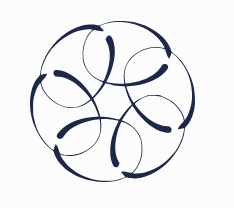
\includegraphics[width=0.4\textwidth]{logo-white.png}\par\vspace{1cm}
    {\scshape\LARGE Software Requirements Specifications\par}
    \vspace{1.5cm}
    {\huge\bfseries Occupi - Office Capacity Predictor\par}
    \vspace{2.5cm}
    \begin{tabular}{|c|c|}
        \hline
        \textbf{Name}      & \textbf{Student Number} \\
        \hline
        Rethakgetse Manaka & u22491032               \\
        Kamogelo Moeketse  & u22623478               \\
        Michael Chinyama   & u21546551               \\
        Tinashe Austin     & u21564176               \\
        Carey Mokou        & u21631532               \\
        \hline
    \end{tabular}
    \vfill
    {\large September 01, 2024\par}
\end{titlepage}

\tableofcontents
\pagebreak

%%%%%%%%%%%%%%%%%%%%%%%%%%%%%%%%%%%%%%%%%%%%%%%%%%%%%%%%
%                MAIN DOCUMENT CONTENT                 %
%%%%%%%%%%%%%%%%%%%%%%%%%%%%%%%%%%%%%%%%%%%%%%%%%%%%%%%%

\section*{Introduction}
\addcontentsline{toc}{section}{Introduction}
The Occupi-Office Capacity Management system is designed to revolutionize the way office space is managed by integrating advanced Machine Learning and predictive models. This innovative system addresses the challenge of efficiently managing office occupancy by providing real-time updates on the current capacity and predicting future occupancy trends.

By leveraging historical data and real-time inputs, the Occupi system enables office managers to make informed decisions about space utilization. It not only provides immediate insights into current occupancy levels but also offers longer-term predictions, facilitating better planning and allocation of resources. This planning capability allows the system to enhance its predictive accuracy over time, creating a dynamic and responsive tool for office capacity management.

The system benefits both daily users and office owners. Employees and visitors can access real-time updates on the current office capacity, ensuring they are aware of occupancy levels before arriving. Office managers and owners receive detailed predictions on future capacity, empowering them to optimize space usage, plan for peak periods, and enhance overall office efficiency.

In summary, the Occupi-Office Capacity Management system introduces a data-driven approach to managing office space, offering both immediate and long-term solutions to enhance occupancy management and improve office operations.

\section*{Purpose and Vision}
\addcontentsline{toc}{section}{Purpose and Vision}
The Occupi-Office Capacity Management system aims to revolutionize office space management by integrating advanced Machine Learning and predictive models. The system addresses the challenge of efficiently managing office occupancy by providing real-time updates on current capacity and predicting future occupancy trends. This enables office managers to make informed decisions about space utilization, ensuring optimal use of office resources.

The vision of the Occupi-Office Capacity Management system is to create a dynamic and responsive tool that benefits both daily users and office owners. By leveraging historical data and real-time inputs, the system offers immediate insights into current occupancy levels and detailed predictions for future capacity. This facilitates better planning and resource allocation, allowing the system to enhance its predictive accuracy over time. Ultimately, the system seeks to introduce a data-driven approach to office capacity management, improving office operations and space efficiency.

\pagebreak

\section*{Specifications}
\addcontentsline{toc}{section}{Specifications}

\subsection*{System Requirements}
\addcontentsline{toc}{subsection}{System Requirements}
Occupi is compatible with the following operating systems:
\begin{itemize}
    \item Windows
    \item Linux
    \item MacOS
    \item Android
    \item iOS
\end{itemize}
Internet connection is required for the system to function optimally.

\pagebreak

\section*{User Stories and Characteristics}
\addcontentsline{toc}{section}{User Stories and Characteristics}

\subsection*{Characteristics}
\addcontentsline{toc}{subsection}{Characteristics}

\paragraph{Employees}
Employees are the primary users of the Occupi-Office Capacity Management system. Their main goal is to efficiently manage their work schedules by leveraging real-time occupancy data and predictions.

\begin{itemize}
    \item \textbf{Check-In:} Employees want to use the app to check in when they arrive at the office, providing the system with accurate occupancy data.
    \item \textbf{View Current Office Capacity:} Employees want to use the system to quickly view the current number of people in the office through the app, helping them decide when to come in or find a less crowded time.
    \item \textbf{Plan Visits:} By accessing occupancy predictions, employees want to plan their visits around expected busy times, enhancing their productivity and ensuring a comfortable working environment.
    \item \textbf{Notifications and Alerts:} Employees want to receive notifications about significant changes in occupancy or office conditions, such as reaching maximum capacity or scheduled maintenance.
\end{itemize}

\paragraph{Managers}
Managers use the Occupi system to make strategic decisions regarding office space utilization and to ensure a smooth operation of the office environment. Managers want to manage their teams effectively and optimize office resources.

\begin{itemize}
    \item \textbf{Historical Trends:} Managers want to access detailed historical data on office occupancy, helping them identify patterns and trends over time.
    \item \textbf{Space Planning:} Using predictions and historical data, managers want to plan the allocation of office space, schedule shifts, and manage peak times effectively.
    \item \textbf{Reporting:} Managers want to generate reports on office usage, occupancy trends, and space efficiency to inform higher-level strategic decisions.
    \item \textbf{Team Management:} Managers want to generate reports on team attendance rates, productivity, and collaboration patterns, helping them optimize team performance and office layout.
\end{itemize}

\paragraph{System Administrators}
System Administrators are responsible for maintaining the overall functionality, data integrity, and performance of the Occupi system.

\begin{itemize}
    \item \textbf{Data Accuracy:} Administrators want to ensure that the data collected by the sensors and other devices is accurate and reliable.
    \item \textbf{System Performance:} Administrators want to monitor system performance, addressing any issues that arise and ensuring that the application runs smoothly.
    \item \textbf{Security:} Administrators want to manage the security of the system, including user access controls, data encryption, and compliance with relevant data protection regulations.
    \item \textbf{Maintenance and Updates:} They perform regular maintenance and updates to the system, ensuring it remains up-to-date with the latest features and security patches.
    \item \textbf{Technical Support:} Provide technical support to other users, troubleshooting issues and providing guidance on using the system effectively.
\end{itemize}

\pagebreak

\subsection*{Stories}
\addcontentsline{toc}{subsection}{Stories}

\paragraph{Employees}
\begin{itemize}
    \item As an employee, I want to log in using my credentials to access the Occupi system.
    \item As an employee, I want to check in when I arrive at the office to update the occupancy data.
    \item As an employee, I want to see the real-time office capacity so that I can decide whether to come to the office.
    \item As an employee, I want to view predicted office capacity for the next two days so that I can plan my office visits accordingly.
    \item As an employee, I want to update my profile information so that my contact details and preferences are accurate.
    \item As an employee, I want to receive notifications about office capacity updates so that I am informed if the office is full.
    \item As an employee, I want to navigate the app easily so that I can find information quickly.
    \item As an employee, I want to use the application in my preferred language so that I can navigate it easily.
    \item As an employee, I want to search for occupancy data by date so that I can find specific information quickly.
\end{itemize}

\paragraph{Managers}
\begin{itemize}
    \item As a manager, I want to view historical occupancy data so that I can identify trends and patterns.
    \item As a manager, I want to generate reports on office occupancy so that I can make informed decisions.
    \item As a manager, I want to receive alerts about office capacity changes so that I can respond quickly.
    \item As a manager, I want to view team attendance rates so that I can optimize team performance.
    \item As a manager, I want to export occupancy data so that I can analyze it externally or share it with stakeholders.
    \item As a manager, I want to search for occupancy data by date so that I can quickly retrieve specific information for analysis or reporting.
    \item As a manager, I want to see visual representations of historical data so that I can understand trends better.
\end{itemize}

\pagebreak

\section*{Functional Requirements}
\addcontentsline{toc}{section}{Functional Requirements}

\subsection*{Requirements}
\addcontentsline{toc}{subsection}{Requirements}
Requirements with a \textbf{*} next to it represent optional and \textit{nice-to-have} requirements.

\begin{enumerate}[label=\arabic*.]
    \item Provide a secure authentication process.
    \begin{enumerate}
        \item Users must be able to log in using their credentials.
        \item Users must be able to log in using their Deloitte email address and password.
        \item Users must be able to log out of the system.
        \item Users must be able to reset their password.
        \item Users onboard using an OTP that expires after 60 minutes.
    \end{enumerate}
    
    \item Provide a user-friendly interface.
    \begin{enumerate}
        \item Users must be able to navigate the app easily.
        \item Users must be able to search for information quickly.
        \item Users must be able to use the app in their preferred language.
        \item Users must be able to choose between different themes: 'Light' and 'Dark'.
    \end{enumerate}
    
    \item Provide real-time office capacity updates.
    \begin{enumerate}
        \item Users must be able to check in when they arrive at the office.
        \item Users must be able to view the current office capacity.
        \item Users must be able to receive notifications about office capacity updates.
    \end{enumerate}
    
    \item Provide office capacity predictions.
    \begin{enumerate}
        \item Users must be able to view predicted office capacity for the next two days.
        \item Users must be able to plan their office visits accordingly.
    \end{enumerate}
    
    \item Provide historical occupancy data.
    \begin{enumerate}
        \item Managers must be able to view historical occupancy data.
        \item Managers must be able to identify trends and patterns.
    \end{enumerate}
    
    \item Generate reports on office occupancy.
    \begin{enumerate}
        \item Managers must be able to generate reports on office occupancy for the past week, month, and year.
        \item Managers must be able to generate reports on team attendance rates, both for the past periods and for specific individuals or dates.
    \end{enumerate}
    
    \item Manage user access controls.
    \begin{enumerate}
        \item System administrators must be able to manage user access controls.
        \item System administrators must be able to specify and assign user roles.
        \item System administrators must be able to revoke user access.
        \item System administrators must be able to ensure data security.
    \end{enumerate}
    
    \item Provide booking functionality.
    \begin{enumerate}
        \item Users must be able to book specific rooms for specific time periods.
        \item Users must be able to view room availability.
        \item Users must be able to cancel bookings.
        \item Users must be able to invite other users to join a booking.
    \end{enumerate}
    
    \item Provide check-in functionality.
    \begin{enumerate}
        \item Users must be able to check in for a specific booking.
        \item Users must be able to check in using booking details and credentials.
        \item The system must detect that users are checking in from a specific location.
        \item The system must implement automatic check-out.
    \end{enumerate}

    \item Provide notifications.
    \begin{enumerate}
        \item Users must be able to receive notifications about maintenance or capacity updates.
        \item Users must be able to receive notifications about their bookings.
    \end{enumerate}
\end{enumerate}

\subsection*{Subsystems}
\addcontentsline{toc}{subsection}{Subsystems}
The Occupi system is divided into several subsystems to manage different aspects of functionality and data handling.

\begin{enumerate}
    \item User Management Subsystem
    \item Profile Management Subsystem
    \item Predictive Model to Graph Subsystem
    \item Security Management Subsystem
    \item Room Management Subsystem
    \item Analytics and Reporting Subsystem
\end{enumerate}

\subsubsection*{User Management Subsystem}
This subsystem manages all aspects of user accounts, including registration, authentication, and role-based access controls (RBAC). It ensures that users can log in, update their profiles, and access specific features based on their assigned roles.

\subsubsection*{Profile Management Subsystem}
This subsystem handles all user profile-related data, including preferences, language settings, and personal details. It allows users to update their profiles and ensures that profile information is accurate and consistent.

\subsubsection*{Predictive Model to Graph Subsystem}
This subsystem is responsible for generating occupancy predictions based on historical data and real-time inputs. It communicates with the AI model to fetch predictions and then renders the predictions visually in graphs and charts for easier interpretation by the user.

\subsubsection*{Security Management Subsystem}
The security subsystem handles encryption, user authentication, and data protection. It ensures compliance with industry standards like OAuth 2.0 for secure authorization and TLS 1.2+ for data in transit.

\subsubsection*{Room Management Subsystem}
The room management subsystem allows users to book office spaces and meeting rooms. It manages availability, booking times, and room capacity, ensuring users can efficiently manage space resources.

\subsubsection*{Analytics and Reporting Subsystem}
This subsystem enables managers to generate detailed reports on office capacity, team attendance, and historical trends. It provides customizable reporting options for both short-term and long-term analysis.

\pagebreak


\subsection*{Use Case Diagrams}
\addcontentsline{toc}{subsection}{Use Case Diagrams}

% Placeholder for diagrams, include images using \includegraphics
\subsubsection*{User Management Subsystem}
\begin{figure}[htbp]
    \centering
    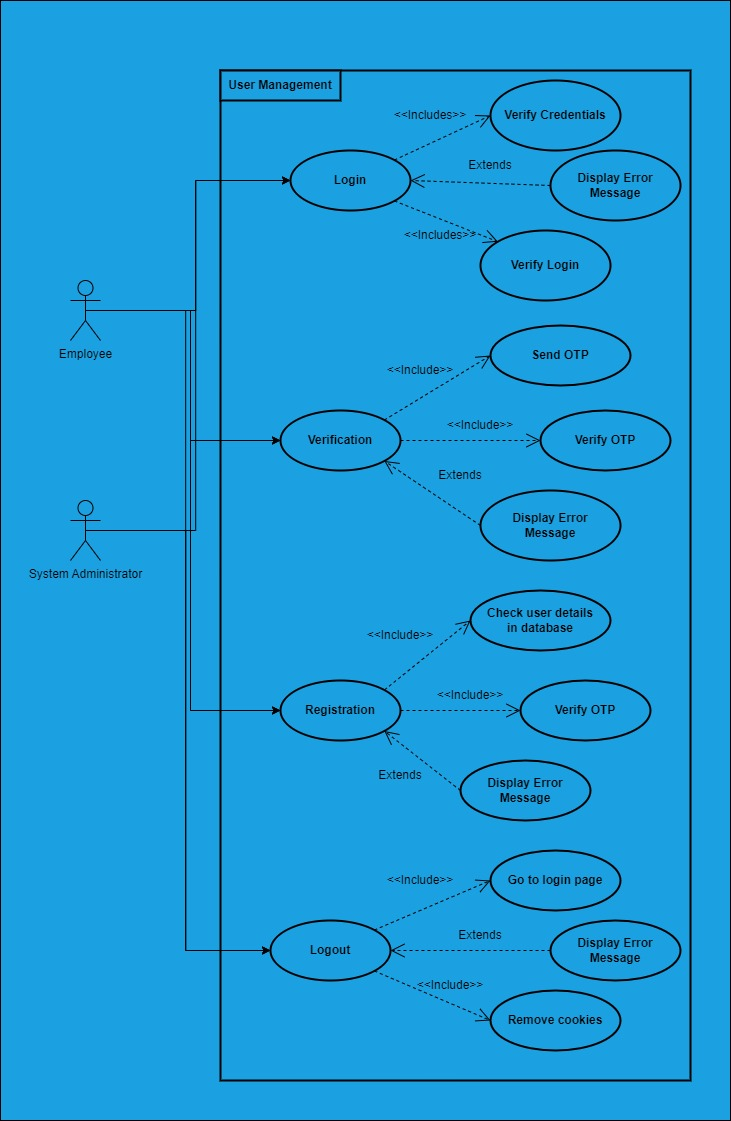
\includegraphics[width=0.7\textwidth]{User_Management.jpg}
    \caption{User Management Subsystem}
\end{figure}

\pagebreak
\subsubsection*{Profile Management Subsystem}
\begin{figure}[htbp]
    \centering
    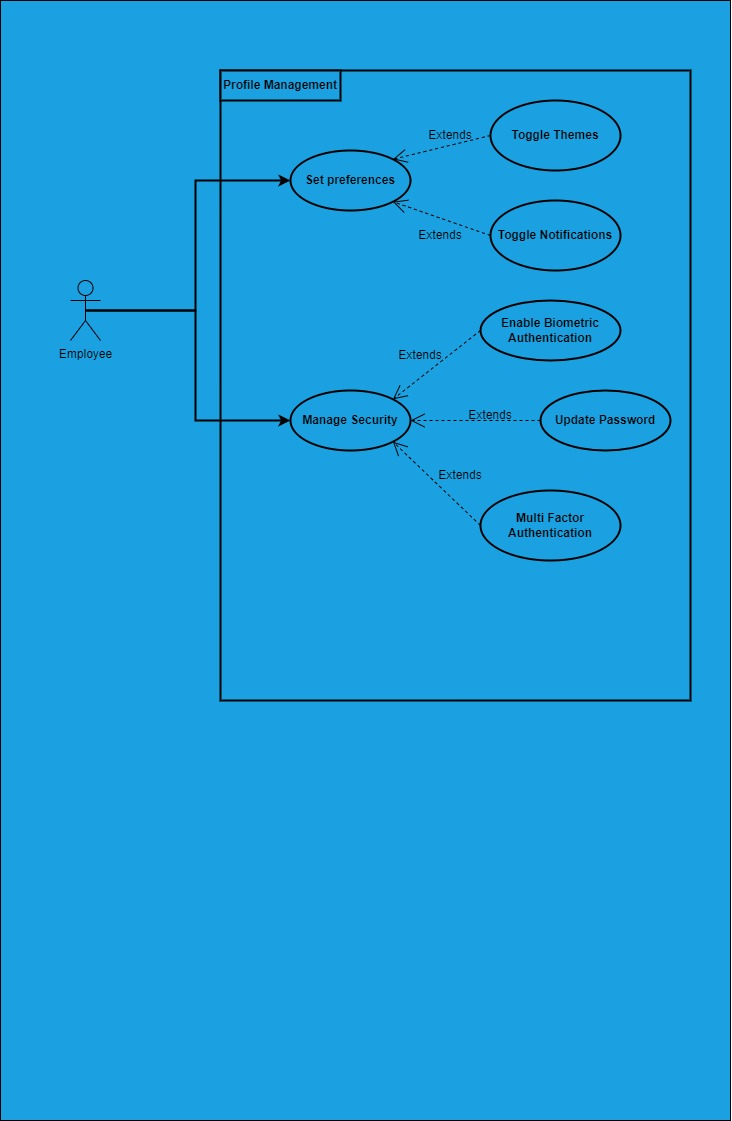
\includegraphics[width=0.7\textwidth]{Profile_Management_2.jpg}
    \caption{User Management Subsystem}
\end{figure}
\pagebreak

\subsubsection*{Predictive Model to Graph Subsystem}
\begin{figure}[htbp]
    \centering
    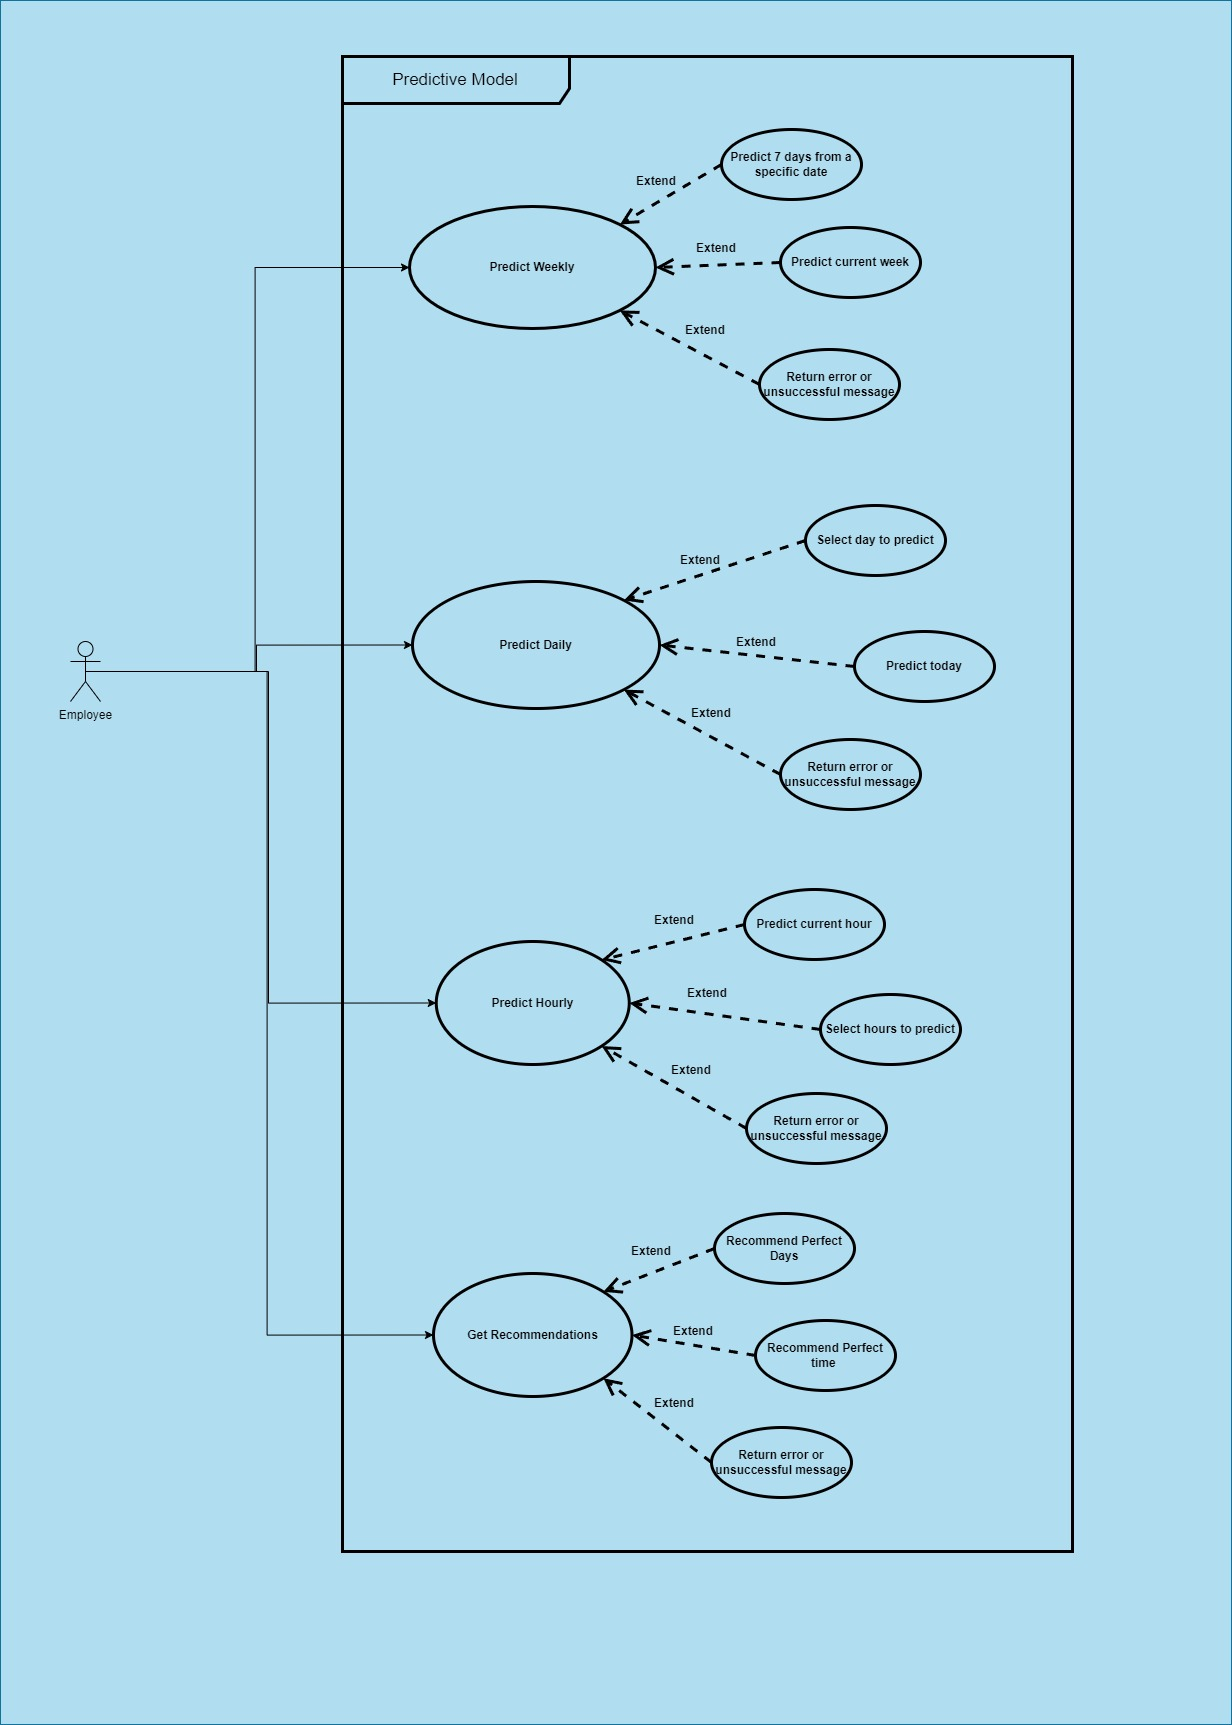
\includegraphics[width=0.7\textwidth]{Predictive_Model_Use_Case.jpg}
    \caption{User Management Subsystem}
\end{figure}
\pagebreak
\subsubsection*{Security Management Subsystem}
\begin{figure}[htbp]
    \centering
    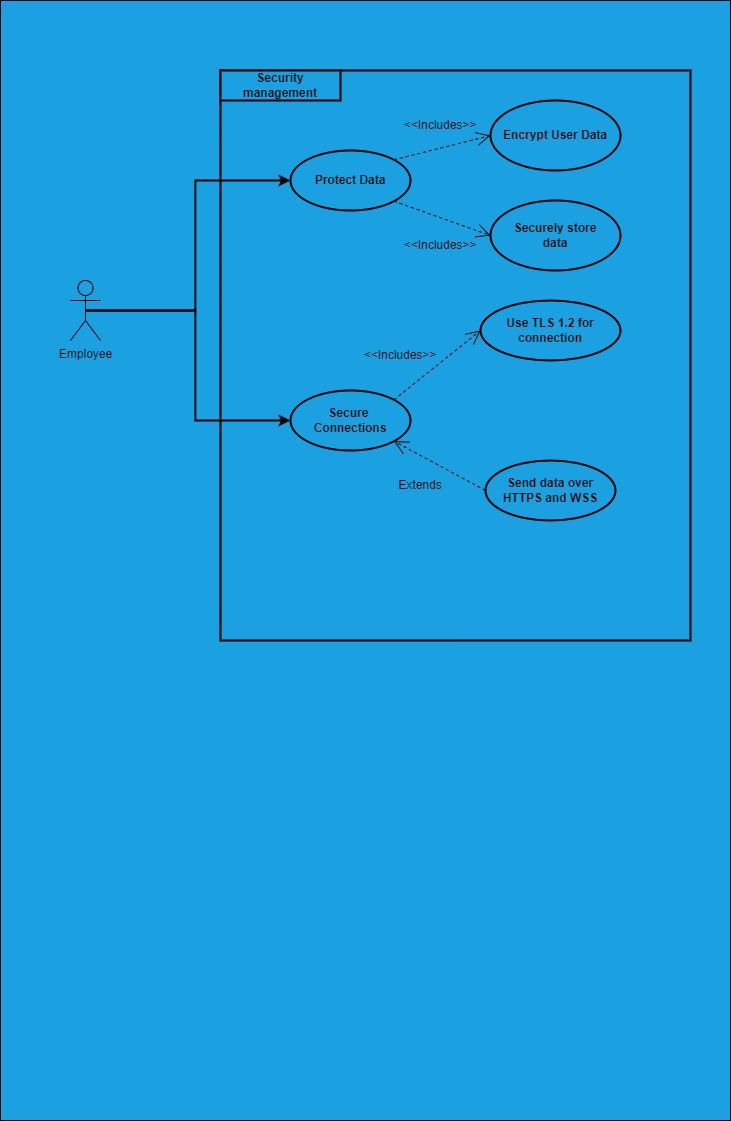
\includegraphics[width=0.7\textwidth]{Security.jpg}
    \caption{User Management Subsystem}
\end{figure}
\pagebreak
\subsubsection*{Room Management Subsystem}
\begin{figure}[htbp]
    \centering
    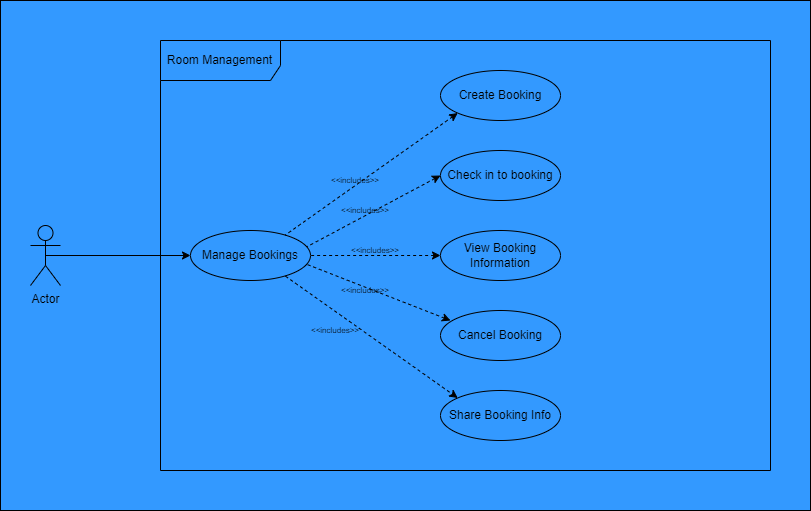
\includegraphics[width=0.7\textwidth]{Room_Management.png}
    \caption{Room Management Subsystem}
\end{figure}
\pagebreak
\subsubsection*{Analytics and Reporting Subsystem}
\begin{figure}[htbp]
    \centering
    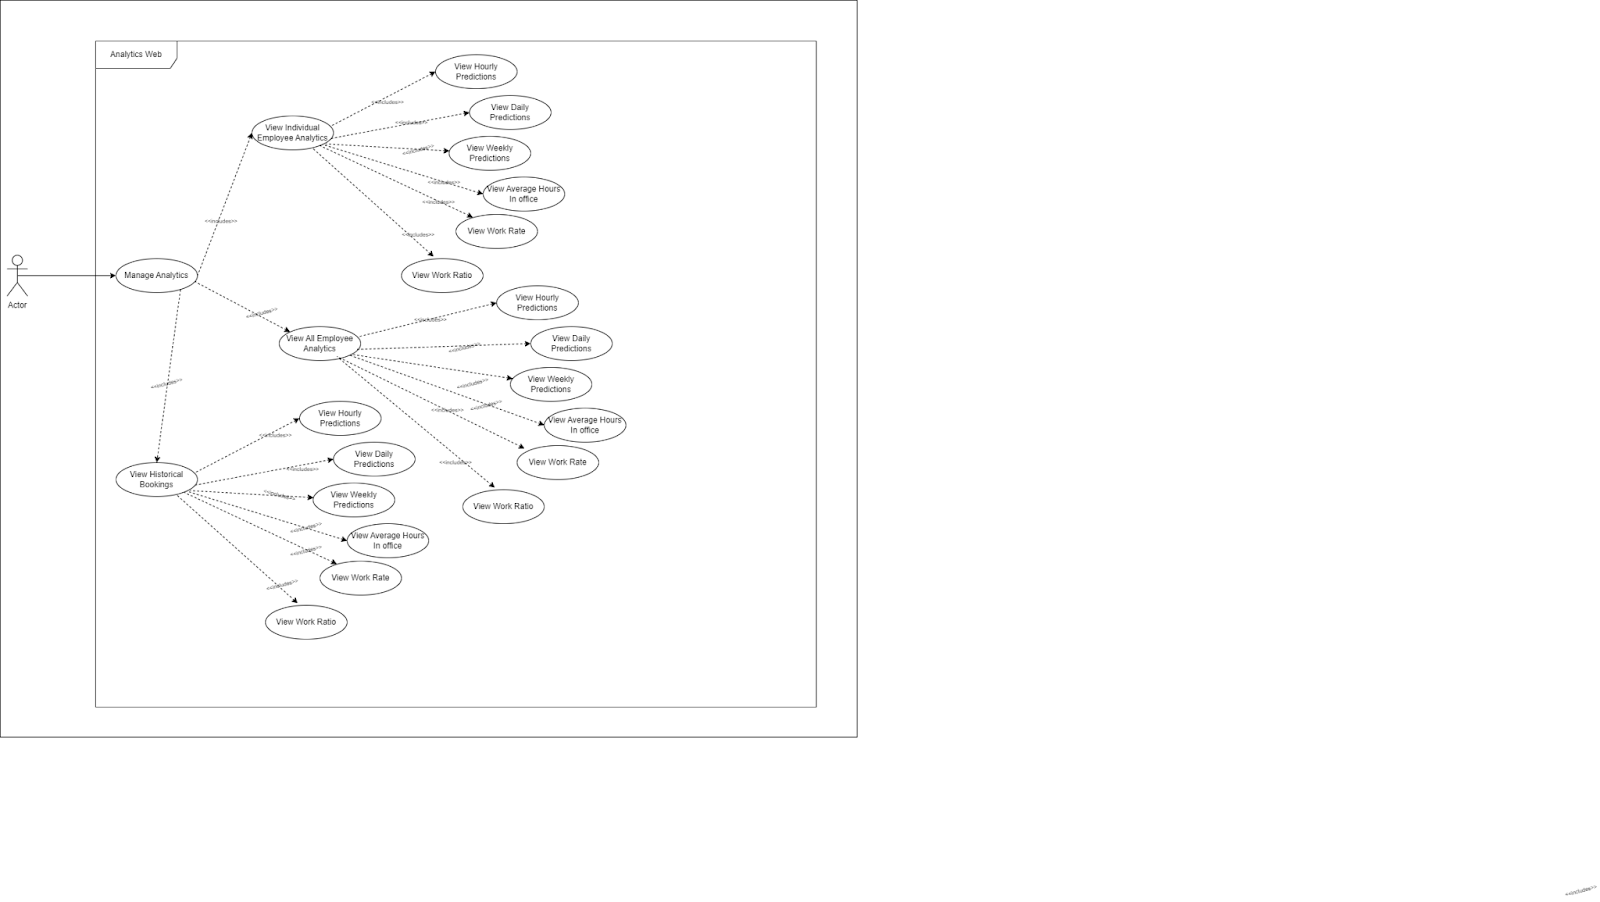
\includegraphics[width=1.0\textwidth]{Analytics and reporting.png}
    \caption{Analytics and Reporting Subsystem}
\end{figure}

\pagebreak

\section*{Quality Requirements}
\addcontentsline{toc}{section}{Quality Requirements}

\subsection*{Performance}
The performance of the Occupi system is critical to its success. The system will be accessed by a large number of users, and it must be able to handle high traffic loads without slowing down or crashing. The system should respond quickly to user requests, providing real-time updates on office capacity and occupancy predictions. To ensure optimal performance, the system should be able to scale horizontally to accommodate additional users and data. The system should also handle peak loads during busy periods, such as the start and end of the workday. Performance testing should be conducted regularly to identify and address any bottlenecks or issues that may arise.

\subsection*{Reliability}
The reliability of the Occupi system is essential to ensure that users can access the system when they need it. The only acceptable downtime is during scheduled maintenance. The system should be designed with redundancy and failover mechanisms to prevent downtime. Regular backups of data should be performed to prevent data loss in case of system failure. Data should be backed up every 7 days and be recoverable within 24 hours. Additionally, the system should be monitored for performance and availability, with alerts sent to administrators if issues are detected.

\subsection*{Scalability}
The Occupi system should be able to scale to accommodate additional users, data, and features as needed. The system should be designed to support horizontal scaling, allowing for the addition of servers to manage increased traffic and data without affecting performance. Vertical scaling should also be supported, allowing individual components to be upgraded to handle increased loads.

\subsection*{Security}
The security of the Occupi system is paramount to protect user data and ensure the integrity of the system. The system should implement strong encryption protocols to protect data in transit and at rest. User authentication should be implemented to ensure that only authorized users access the system, with role-based access controls (RBAC) in place to restrict access to sensitive data and features. Re-authentication should occur every 90 days using OAuth 2.0 for secure authorization, and domain-specific access should be implemented to ensure that only users with the correct domain access the system.

\subsection*{Usability}
The Occupi system should be easy to use and navigate, with an intuitive interface that allows users to find information quickly. The system should follow Deloitte's design cues to ensure consistency across all platforms. It should also be responsive, adapting to different screen sizes and devices to provide a seamless user experience. User feedback should be collected regularly to identify areas for improvement and enhance the usability of the system.

\subsection*{Compliance}
Due to personal data being collected, the Occupi system must comply with relevant data protection regulations, such as the Protection of Personal Information Act (POPIA). The system should implement data protection measures to ensure that user data is secure and protected from unauthorized access. Compliance with industry standards and best practices for data security and privacy is essential. Regular audits and reviews should be conducted to ensure ongoing compliance with Deloitte’s data protection policies and relevant regulations.

\subsection*{Interoperability}
The Occupi system should integrate seamlessly with Deloitte’s existing building access control systems. This integration allows the system to automatically update occupancy data based on user check-ins and check-outs. The system should be compatible with a wide range of devices and platforms, including desktops, laptops, tablets, and smartphones. The system should also integrate with the building's network infrastructure to ensure that users are checking in from the correct location.

\subsection*{Compatibility}
The Occupi system should be compatible with the following operating systems:
\begin{itemize}
    \item Windows
    \item Linux
    \item MacOS
    \item Android
    \item iOS
\end{itemize}
It should also be accessible from any device with an internet connection, allowing users to access real-time updates on office capacity and occupancy predictions.

\pagebreak

\section*{Design Strategy}
\addcontentsline{toc}{section}{Design Strategy}

The architectural design strategy for the development of Occupi involves the following: Agile and Decomposition.

\subsection*{Agile strategy}
This strategy focuses on iterative development, continuous feedback from clients, cross-functional teams as well as adaptability. Iterative development involves work being divided into small, manageable increments. This aids the development process of the project in that it allows the team to break parts of the projects apart and focus on one part at a time. This makes the project more manageable. Continuous feedback from the client helps to ensure that the product meets their needs. This helps to prevent the team from diverting from the requirements of the product.

\subsection*{Decomposition Strategy}
This strategy emphasizes breaking down complex projects into smaller, more manageable components. Decomposition involves dividing the project into discrete, self-contained modules or tasks. This approach enhances the development process by allowing the team to concentrate on individual segments, making the overall project easier to handle. Each module can be developed, tested, and refined independently before integrating it into the larger system. Regular assessments and adjustments at each stage ensure that each part aligns with the overall project goals. This strategy minimizes risks, improves resource allocation, and ensures that the final product meets the desired standards and specifications.

\section*{Quality Requirements}
\addcontentsline{toc}{section}{Quality Requirements}

\subsection*{Performance}
\textbf{Description:} The performance of the Occupi system is critical to its success. The system will be accessed by a large number of users, and it must be able to handle high traffic loads without slowing down or crashing. The system should respond quickly to user requests, providing real-time updates on office capacity and occupancy predictions. To ensure optimal performance, the system should be able to scale horizontally to accommodate additional users and data. The system should also be able to manage peak loads during busy periods, such as the start and end of the workday. Performance testing should be conducted regularly to identify and address any bottlenecks or issues that may arise.

\textbf{Quantification:} To quantify the performance of Occupi, several key metrics are essential, and each will be measured using specific methods. The system should support at least 10,000 concurrent users. It must process a minimum of 1,000 requests per second. Horizontal scaling should double system capacity, verified by load tests conducted before and after scaling. Peak load conditions should keep CPU and memory usage below 80%. Update latency for occupancy data should be within 1 second, and data freshness should be ensured with updates every minute, both measurable with automated scripts. Lastly, uptime should be maintained at 99.9% and error rates kept below 0.1%. Regular performance testing and monitoring of these metrics will ensure the system's reliability and user satisfaction.

\textbf{Architectural Strategy:} Spread Load, Reduce Load

\subsection*{Reliability}
\textbf{Description:} The reliability of the Occupi system is essential to ensure that users can access the system when they need it. The only time that is acceptable for the system to be down is during maintenance. To ensure reliability, the system should be designed with redundancy and failover mechanisms to prevent downtime. Regular backups of data should be performed to prevent data loss in the event of a system failure. Data should be backed up every 7 days and be recoverable within 24 hours. The system should also be monitored for performance and availability, with alerts sent to administrators if any issues are detected.

\textbf{Quantification:} To quantify the reliability of the Occupi system, several key metrics and measures are necessary. The system's uptime should be maintained at 99%, allowing for minimal downtime, which is only acceptable during scheduled maintenance. Redundancy and failover mechanisms should ensure that any single point of failure does not lead to system-wide downtime, aiming for seamless failover within 1 minute. Regular backups should be performed every 7 days to prevent data loss, with a goal of 100% successful backup completion. In case of a system failure, data recovery should be achievable within 24 hours, ensuring minimal disruption. The system should be monitored continuously for performance and availability with response time for alerts set to within 5 minutes. Additionally, administrators should receive immediate alerts if the system's performance deviates from the expected norms, with an aim to resolve issues within 1 hour of detection. Regular performance and reliability testing should be conducted to validate these measures and ensure the system meets these stringent reliability requirements.

\textbf{Architectural Strategy:} Logging, Testing framework, Passive Redundancy

\subsection*{Security}
\textbf{Description:} The security of the Occupi system is paramount to protect user data and ensure the integrity of the system. Due to the system collecting data on users, it is important that the system is secure. The system should implement strong encryption to protect data in transit and at rest. User authentication should be implemented to ensure that only authorized users can access the system. Access controls should be in place to restrict user access to sensitive data and features. User authentication should take place every 90 days. User authentication systems such as OAuth should be implemented to ensure that user data is secure. Domain specific access should be implemented to ensure that only users with the correct domain can access the system.

\textbf{Quantification:} To quantify the security of the Occupi system, several key metrics and methods are essential. All data transmitted over the network must be encrypted using TLS 1.2 or higher, and 100% of stored data should be encrypted using AES-256. User re-authentication should occur every 90 days, with a compliance rate of 100%, utilizing OAuth 2.0 for secure authorization. Implement role-based access controls (RBAC) to restrict access to sensitive data and features, ensuring 100% compliance with access control policies. Only users with verified domains should access the system, aiming for a 100% verification rate. Real-time intrusion detection systems should monitor for security breaches with a response time under 5 minutes, and audit logs should retain 100% of access and changes to sensitive data for at least 1 year.

\textbf{Architectural Strategy:} Limit Exposure, Limit access, Event Logging

\subsection*{Usability}
\textbf{Description:} The Occupi system should be easy to use and navigate, with an intuitive interface that allows users to find information quickly and easily. The system should be accessible and user friendly, with clear instructions and guidance provided to help users understand how to use the system. The system should follow Deloitte design cues and be consistent across all platforms. The system should also be responsive, adapting to different screen sizes and devices to provide a consistent user experience. User feedback should be collected regularly to identify areas for improvement and enhance the usability of the system.

\textbf{Quantification:} To quantify the usability of the Occupi system, several key metrics are essential. Conduct regular audits to ensure 100% adherence to Deloitte design cues across all platforms and test the system on various devices to maintain a consistent user experience with 0% critical issues. The system's page load time should average under 2 seconds, with 100% of the interface adapting appropriately to different screen sizes and devices. Collect user feedback at least quarterly, aiming to address and implement changes within 2 months and achieve a 90% or higher resolution rate. By monitoring these metrics, the usability of the Occupi system can be quantified and continuously improved.

\textbf{Architectural Strategy:} Support User Initiative (Cancel, Undo)

\subsection*{Compliance}
\textbf{Description:} Due to personal data being collected, the Occupi system must comply with relevant data protection regulations, such as the Protection of Personal Information Act (POPIA). The system should implement data protection measures to ensure that user data is secure and protected from unauthorized access. The system should also comply with industry standards and best practices for data security and privacy. Regular audits and reviews should be conducted to ensure that the system remains compliant with Deloitte’s data protection policies and relevant regulations.

\textbf{Quantifiers:} To quantify the compliance and data protection of the Occupi system, conduct compliance audits at least twice a year, aiming for a 100% compliance rate with the Protection of Personal Information Act (POPIA). Ensure 100% of user data is encrypted both in transit (using TLS 1.2 or higher) and at rest (using AES-256), and implement role-based access controls (RBAC) with a 100% compliance rate. Achieve 100% compliance with industry standards such as ISO/IEC 27001 and perform quarterly vulnerability scans, addressing any issues within 30 days. Conduct regular audits and reviews of data protection measures at least quarterly, resolving 100% of identified issues within 60 days. Ensure 100% adherence to Deloitte’s data protection policies and conduct annual data protection and privacy training for all employees with a 100% participation rate.

\textbf{Architectural Strategy:} Security

\subsection*{Results of Penetration Testing}
\href{https://drive.google.com/drive/folders/1iZRAiG3MAeO29Iqtde19l5mjX47NGkFP}{Results to Penetration Testing}

\pagebreak

\section*{Architectural Design \& Patterns}
\addcontentsline{toc}{section}{Architectural Design \& Patterns}

\subsection*{MVC (Model-View-Controller)}
We chose the MVC pattern to separate concerns for user interface, business logic, and data management. The MVC pattern promotes a clean separation of concerns between data management (Model), user interface (View), and application logic (Controller), making our codebase more modular and easier to maintain.

\textbf{Model: Database} - The Model represents the core backend of our system, managing the data and the business logic. It serves as the central source of truth for all other views in the system. In our architecture, the Model includes:
\begin{itemize}
    \item \textbf{MongoDB:} The primary database for storing and retrieving application data. MongoDB's NoSQL structure allows for flexible, scalable, and high-performance data management.
\end{itemize}

\textbf{View: Frontend} - The View is responsible for displaying data to the user and capturing user input. It is the user interface layer of the application. In our architecture, the View includes:
\begin{itemize}
    \item \textbf{Web Frontend (React):} The client-side part of the application for our Management Terminal, built using React. It renders the user interface, allowing users to interact with the system. It displays dashboards and other data visualization elements to assist in understanding office capacity trends.
    \item \textbf{Mobile Frontend (React Native):} The client-side part of the application for mobile users, built using React Native. It provides a seamless and responsive user experience on mobile devices whilst booking, checking in, and viewing office occupancy.
\end{itemize}

\textbf{Controller: AI Model Server} - The Controller acts as an intermediary between the Model and the View. It processes incoming requests, performs operations on the Model, and updates the View accordingly. In our architecture, the Controller includes:
\begin{itemize}
    \item \textbf{Python AI Model:} Integrates AI-related operations such as data processing, making predictions, and providing intelligent responses. This component works closely with the Go server to handle AI tasks.
\end{itemize}

\subsection*{Layered Pattern}
\begin{itemize}
    \item \textbf{Presentation Layer:} Consists of user interfaces, such as the mobile application for employees and the management terminal for managers, handling user input and providing a consistent experience.
    \item \textbf{Application Layer:} Encapsulates business logic related to occupancy tracking, prediction algorithms, and other core functionalities, ensuring separation of concerns.
    \item \textbf{Service Layer:} Includes various services or components responsible for specific tasks like user management, occupancy tracking, and real-time updates, implemented as microservices for scalability.
    \item \textbf{Data Access Layer:} Abstracts data storage mechanisms like MongoDB, providing a consistent interface for interacting with data sources.
    \item \textbf{Security Layer:} Handles authentication, authorization, and data protection, implemented as a cross-cutting concern or separate layer based on complexity.
\end{itemize}

\subsection*{Client-Server Architecture}
\textbf{Client:} The client can forward requests to the backend via multiple endpoints and environments (production or development). The domain registrar handles DNS for clients and forwards requests to the server's IP address.

\textbf{Server:} We use a VM instance acting as a server that listens for incoming requests on port 443 (HTTPS) and serves clients with different content, including documentation, landing page, web app, or API backend. A reverse proxy sits between port 443 and our containers.

\pagebreak
\subsubsection*{Architectural Design Diagram}
\begin{figure}[htbp]
    \centering
    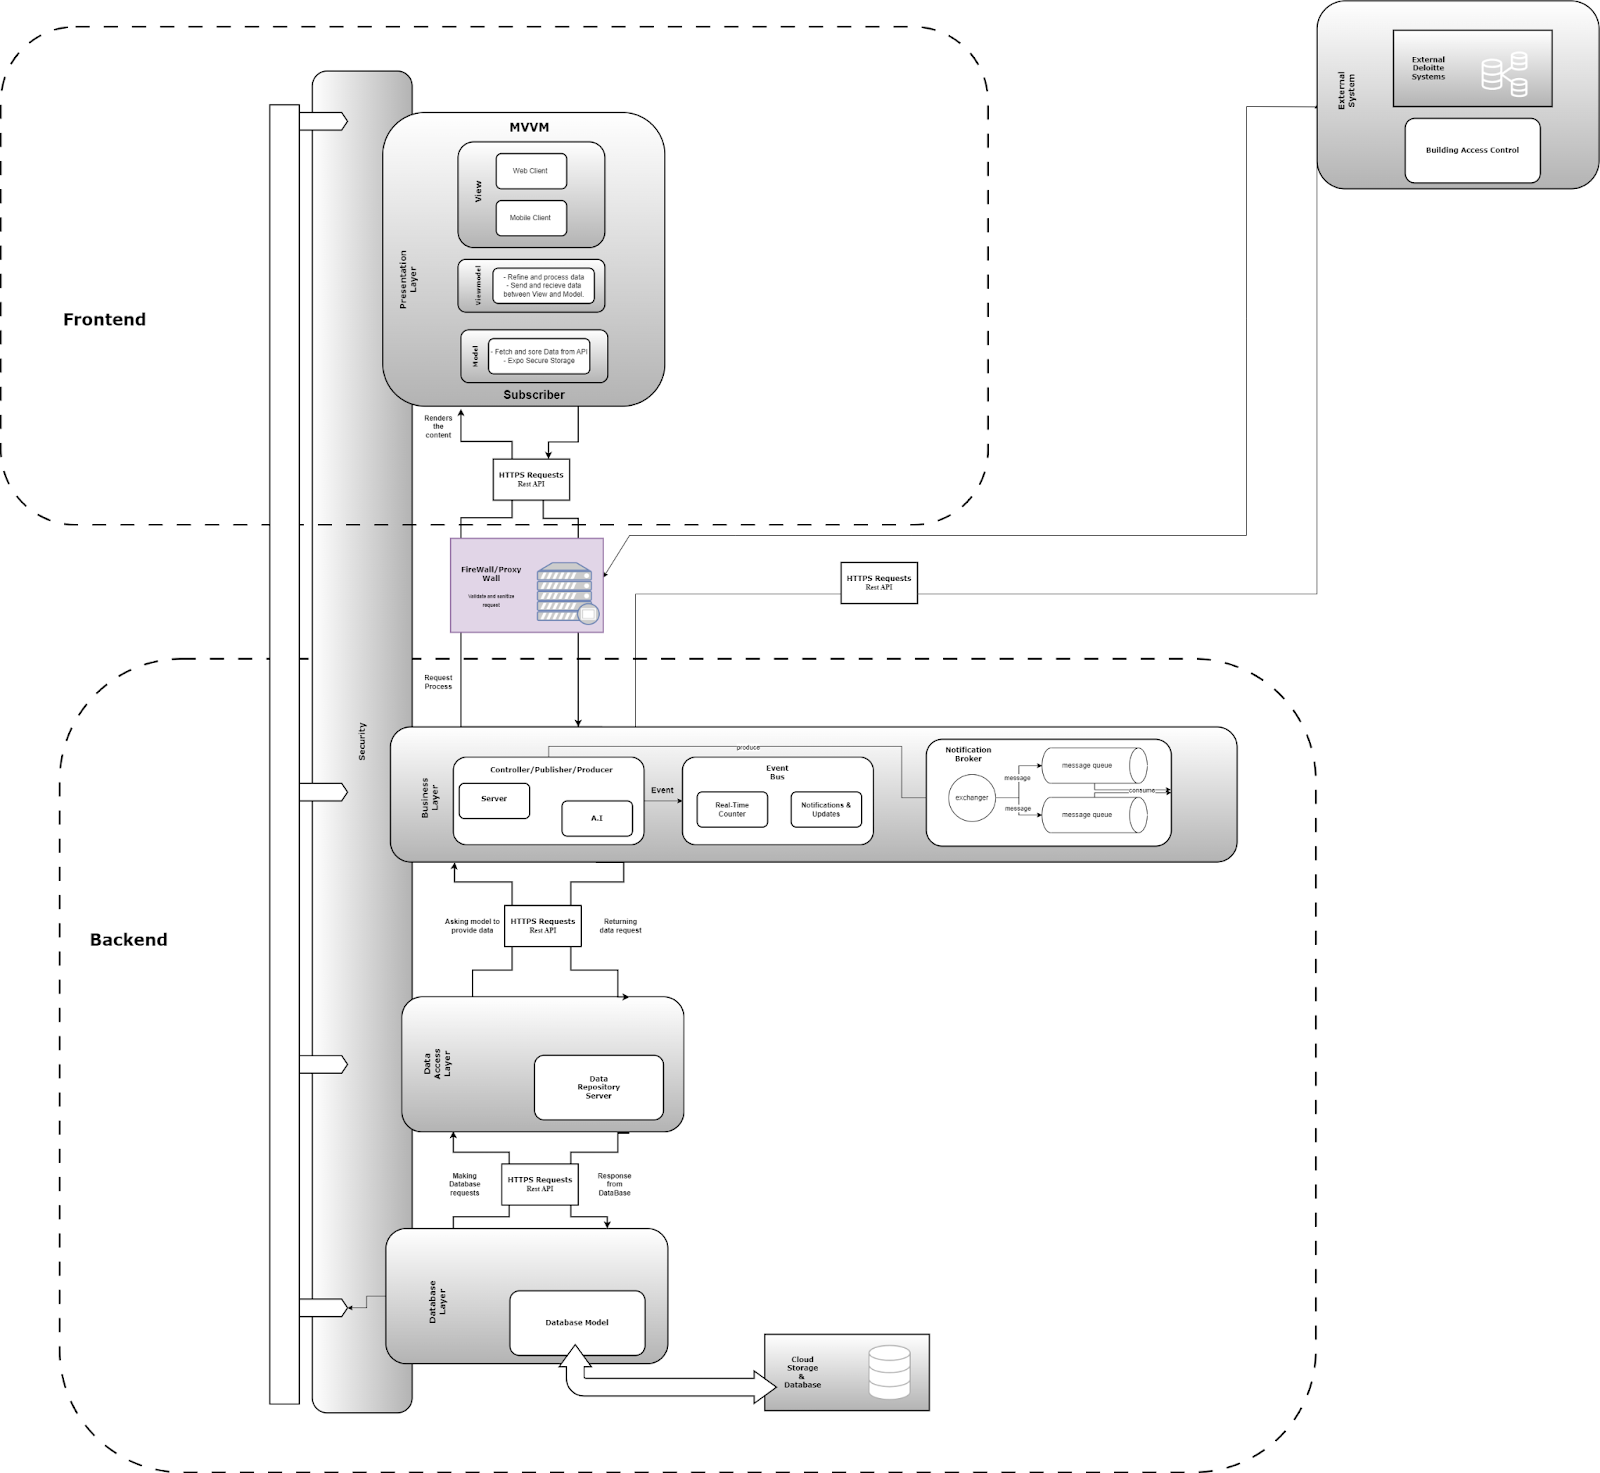
\includegraphics[width=0.8\textwidth]{Architectural Diagram.png}
\end{figure}
\pagebreak

\section*{Technology Choices}
\addcontentsline{toc}{section}{Technology Choices}

\subsection*{For Web-based Development}

\paragraph{React:} A JavaScript library for building user interfaces. It is component-based, which promotes reusability and makes code easier to manage, although the learning curve can be steep for beginners.
\begin{itemize}
    \item \textbf{Pros:}
    \begin{itemize}
        \item Component-based architecture allows for modular and reusable code.
        \item Large ecosystem with a vast array of libraries and tools.
        \item Virtual DOM for efficient rendering and updates.
        \item Supported by a large community and backed by Facebook.
    \end{itemize}
\end{itemize}

\paragraph{Tailwind CSS:} A utility-first CSS framework that allows for highly customizable designs. It can speed up development but may seem verbose for some.
\begin{itemize}
    \item \textbf{Pros:}
    \begin{itemize}
        \item Utility-first approach allows for rapid styling and prototyping.
        \item Highly customizable and flexible.
        \item Promotes consistency and maintainability across projects.
    \end{itemize}
\end{itemize}

\paragraph{Component Libraries (Schadcn, DaisyUI, NextUI, Framer Motion):} These libraries provide pre-built components that speed up development and ensure consistency, though they might limit customization.
\begin{itemize}
    \item \textbf{Pros:}
    \begin{itemize}
        \item Accelerates development by providing pre-built UI components.
        \item Ensures consistent design and styling across the application.
        \item Well-documented and actively maintained by communities.
    \end{itemize}
\end{itemize}

\subsection*{For Mobile Development}

\paragraph{React Native:} A framework for building native apps using React. It allows code sharing between platforms, reducing development time, but may not be as performant as native code for complex apps.
\begin{itemize}
    \item \textbf{Pros:}
    \begin{itemize}
        \item Write once, run anywhere (iOS and Android) with native performance.
        \item Large community and extensive ecosystem of libraries and tools.
        \item Easier learning curve for developers familiar with React.
    \end{itemize}
\end{itemize}

\paragraph{Component Libraries (UI Kitten, GlueStackUI):} Similar to web development, these libraries can speed up mobile app development while ensuring a consistent user experience.
\begin{itemize}
    \item \textbf{Pros:}
    \begin{itemize}
        \item Pre-built components specifically designed for React Native.
        \item Consistent look and feel across platforms.
        \item Actively maintained and well-documented.
    \end{itemize}
\end{itemize}

\subsection*{For Backend Development}

\paragraph{Go:} A statically typed, compiled language that is efficient for building web services and microservices. Its simplicity may limit it for complex applications.
\begin{itemize}
    \item \textbf{Pros:}
    \begin{itemize}
        \item Statically typed language promotes code safety and reliability.
        \item Excellent performance and high concurrency support.
        \item Simple and clean syntax, easy to learn and maintain.
        \item Built-in support for concurrency and parallelism.
    \end{itemize}
\end{itemize}

\paragraph{MongoDB Driver Support:} Enables rapid development and deployment for web services, microservices, and cloud-native apps. However, MongoDB might not be ideal for applications requiring complex transactions.
\begin{itemize}
    \item \textbf{Pros:}
    \begin{itemize}
        \item Flexible and scalable NoSQL database.
        \item Well-suited for distributed systems and cloud-native applications.
    \end{itemize}
\end{itemize}

\paragraph{REST API, JSON Web Tokens (JWTs):} REST is a standard for designing networked applications, while JWTs offer a secure way of transmitting information between parties.
\begin{itemize}
    \item \textbf{Pros:}
    \begin{itemize}
        \item REST APIs provide a widely adopted architectural style for building web services.
        \item JWTs offer a compact and secure way to transmit claims between parties.
        \item Stateless authentication mechanism reduces server-side overhead.
    \end{itemize}
\end{itemize}

\subsection*{Reasons for Frontend}
We chose React for its component-based architecture, which promotes modular and reusable code, alongside Tailwind CSS for rapid styling and customizability. Component libraries such as Schadcn, DaisyUI, and NextUI help accelerate development and maintain a consistent design. This combination ensures a robust and efficient development environment.

\subsection*{Reasons for Backend}
Go was selected for its high concurrency support, simplicity, and efficiency, making it ideal for building scalable web services. MongoDB provides a flexible and scalable NoSQL database, suitable for cloud-native apps. REST APIs and JWTs were chosen for their simplicity and security, ensuring scalability and secure data transmission.

\subsubsection*{Deployment Diagram}
\begin{figure}[htbp]
    \centering
    \includegraphics[width=1\textwidth]{Occupi Deployment model.png}
\end{figure}
\end{document}

